\vspace{-.5cm}
\section{Tool Demonstration}
\label{sec:demo}
\vspace{-.3cm}
In this section, we discuss the main steps of the process that need to be
followed for synthesizing the EARS-CTRL specification into a controller and
validating if the controller behaves as expected.
\vspace{-.3cm}
\subsection{Building a Glossary}
\vspace{-.2cm}
The first step towards writing the controller specifications in natural
language using \textsf{EARS-CTRL} is to define a glossary of terms. 
As is depicted in figure~\ref{fig:glossary_def}, the user is provided with an
editor to define glossary terms for: 1) components that interface with the
controller; 2) sensors and actuators those components make available to the controller; 3) invariant relations
that should hold between the sensor and actuator signals; and 4) for ease of
writing, aliases to formulas involving sensors or actuators.
\vspace{-.2cm}
\begin{figure*}[!h]
\centering
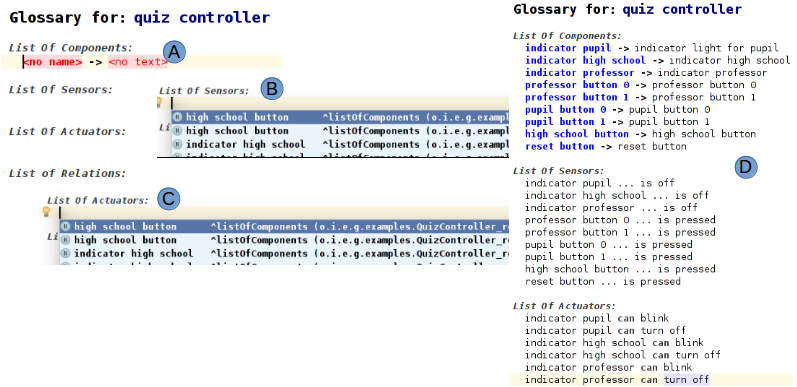
\includegraphics[width=1\textwidth]{./images/QC_Glossary_Def.png}
\caption{Step-by-step glossary building for a Quiz Controller: (\emph{A})
components definition, (\emph{B}) sensors definition, (\emph{C}) actuators
definition and (\emph{D}) completed QC glossary}
\label{fig:glossary_def}
\vspace{-.6cm}
\end{figure*}
\subsection{Building \textsf{EARS-CTRL} requirements for the Quiz Controller}
\vspace{-.2cm}
Figure~\ref{fig:EARS_req} provides the set of steps required to write a set of
EARS requirements. In the projectional editor the user presses the CTRL+Space
key combination to instantiate an EARS-based template that presents a number of
placeholders (\emph{Step A}\levi{fix step A with new editor}). After obtaining
an instance of the EARS template, the user fills in the placeholders with
information coming from the glossary definitions (\emph{Step B}). \emph{Step C}
depicts the complete Quiz Controller specification.
\begin{figure*}[!h]
\centering
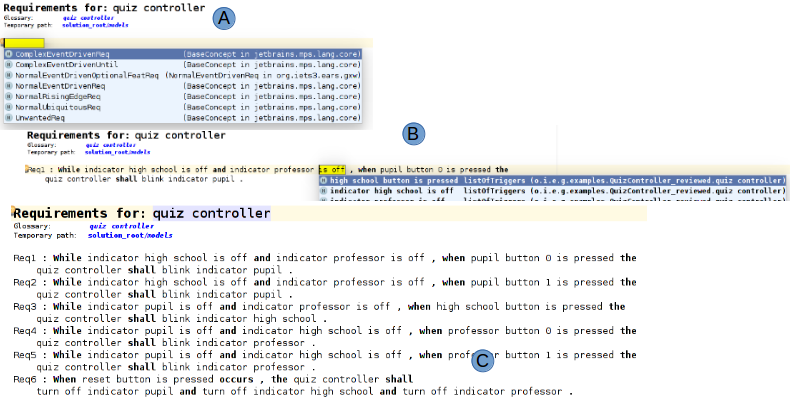
\includegraphics[width=1.2\textwidth]{./images/Req_Spec_Steps.png}
\caption{Step-by-step guidance for building controller requirements in
\textsf{EARS-CTRL}, (\emph{A}) empty instance of EARS template with placeholders, (\emph{B}) filling instance
of an EARS template with information and (\emph{C}) completed EARS Specification
}
\label{fig:EARS_req}
\vspace{-.6cm}
\end{figure*}
\vspace{-.2cm}
\subsection{Synthesizing \textsf{EARS-CTRL} requirements}
\label{SynthReq}
\vspace{-0cm}
Once the requirements for controller are completely specified, the user can
attempt to synthesize the controller. For that the \emph{Transform} intention
can be used by using the \emph{Alt+Enter} keys on the root of the specification
(as shown in \emph{part A} of figure~\ref{fig:Spec_transform}). The generated
output after applying the intention is comprised of: 1) the  \emph{Synchronized
Data Flow} (SFD) diagram containing blocks connected by wires (\emph{part B} of
figure~\ref{fig:Spec_transform}); 2) pseudo code representing the behavior of each of the blocks used
by the synthesized controller (\emph{part C} of
figure~\ref{fig:Spec_transform}); 3) a Simulink block
diagram (\emph{part D} of figure~\ref{fig:Spec_transform}); and 4) empty panel
for performing simulation and test cases generation (\emph{part E} of
figure~\ref{fig:Spec_transform})\levi{fix panel to new version and there is
some confusion here between numbers and letters. Maybe just use letters to
avoid confusion}.
%\vspace{-.7cm}
\begin{figure*}[!h]
\centering
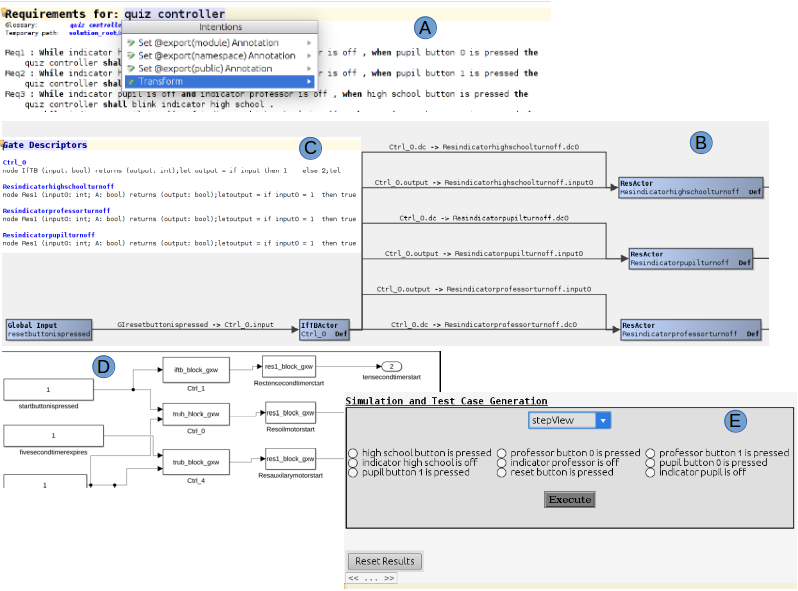
\includegraphics[width=1\textwidth]{./images/Transform.png}
\caption{Controller generation steps: (\emph{A}) applying intention \emph{Alt+Enter},
(\emph{B}) synchronized DFD of the controller (an excerpt), (\emph{C}) pseudo
code representing the behavior of the blocks (an excerpt), (\emph{D})
generated Simulink model (an excerpt) and (\emph{E})
generated empty panel for simulation}
\label{fig:Spec_transform}
\end{figure*}
\vspace{-.5cm}
\subsection{Simulation and Test Cases for Validation of Controller
Behavior\levi{there are too many explanations here. You don't need to explain
what things are, this is already done in the paper. Jut say which steps are
done in the demo!}}
\vspace{-.2cm}
Validation of the generated controller to check if it behaves as expected can be
performed using following techniques: 1) simulating the behavior of the
controller step-by-step; and 2) automatically generating the test cases.
The resulting traces from simulation or test generation are analyzed in order to
check if the controller behaves as expected.
\vspace{-.3cm}
\subsubsection{Simulation}
\vspace{-.2cm}
In order to perform simulation of the generated controller, the user gets the
\textsf{EARS-CTRL} panel (i.e., as a result of applying the \emph{Transform}
intention in section~\ref{SynthReq}) that allows the user to
simulate the controller by providing a sequence of inputs manually.
Figure~\ref{fig:SimulationSteps} shows a panel where outputs (i.e., the results)
can be viewed in a tabular view provided to the user. A \textsf{“Reset Results”}
button enables the user to reset the controller to its initial state. 
\begin{figure*}[!h]
\centering
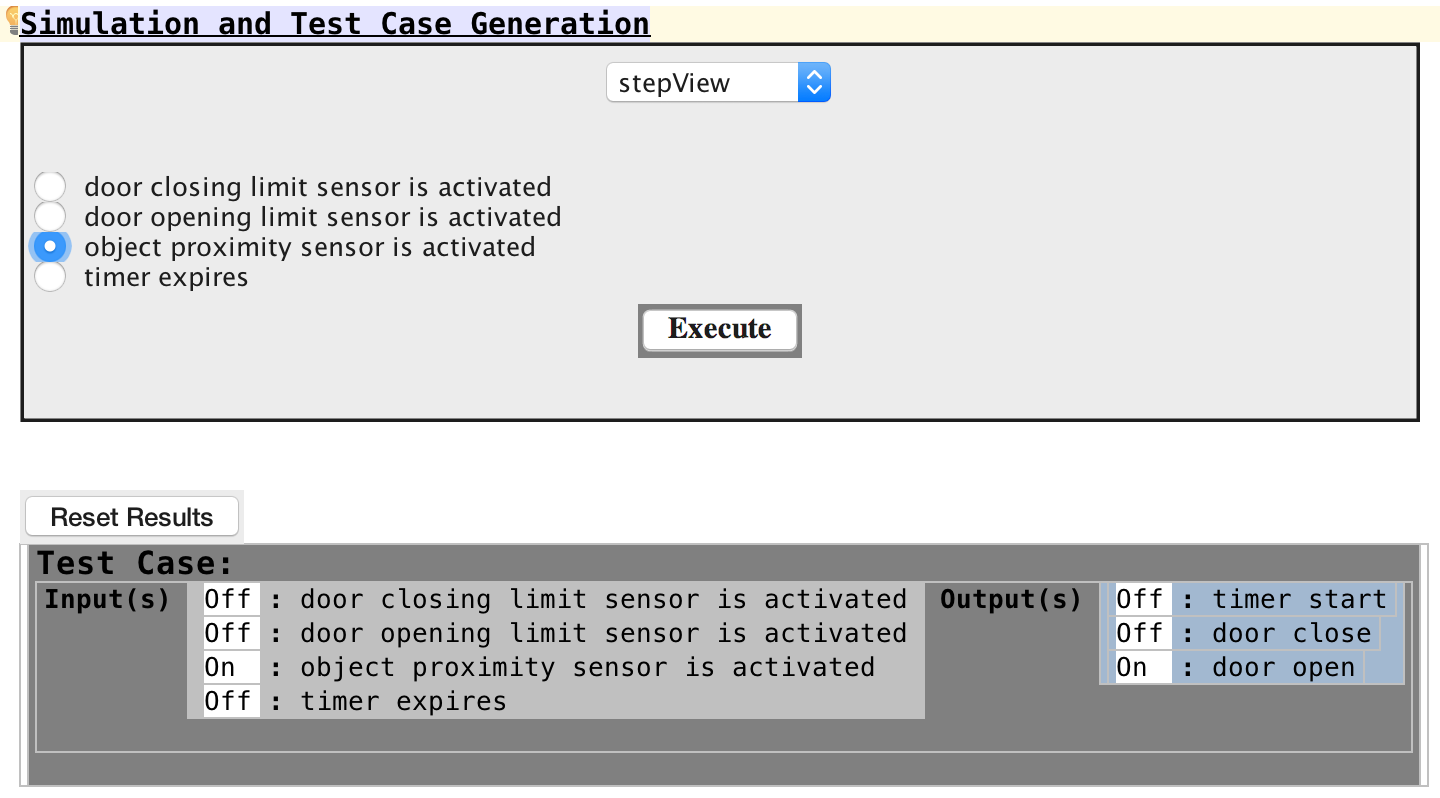
\includegraphics[width=.9\textwidth]{./images/simulation.png}
\caption{A panel for simulation of the generated controller for validation}
\label{fig:SimulationSteps}
\vspace{-.6cm}
\end{figure*}
%\vspace{-.3cm}
\subsubsection{Automatic Test Cases Generation} 
\vspace{-.5cm}
The user can automatically generate test cases
(figure~\ref{fig:TestCaseGeneration}) by setting in the testing parameters.
For the test case generation, the user inputs the
parameters in the \textsf{EARS-CTRL} panel.
The parameters required for test case generation are as follows, 1) \textsf{Test
Sequence Length(integer value)}, 2) \textsf{Allow parallel inputs(true/false)} and 3) \textsf{Allow repeated inputs (true/false)}.